\documentclass[a4paper,oneside]{article}

\usepackage[utf8]{inputenc}
\usepackage[T2A]{fontenc}
\usepackage[english,russian]{babel}

\usepackage{amsmath}
\usepackage{mathtools}
\usepackage{amsfonts}
\usepackage{enumitem}
\usepackage{amsthm}
\usepackage{minted}
\setminted{fontsize=\small, breaklines=true, style=emacs, linenos}
\usepackage{graphicx}
\graphicspath{ {./images/} }
\usepackage{float}

\newtheorem{theorem}{Теорема}[subsection]
\newtheorem*{theorem*}{Теорема}

% --- Определение --- %
\theoremstyle{definition}
\newtheorem{definition}{Определение}[subsection]
\newtheorem*{definition*}{Определение}
% ------------------- %

\title{{Теория кодирования и сжатия информации}\\{Лабораторная работа №10}}
\author{Гущин Андрей, 431 группа, 1 подгруппа}
\date{\the\year{} г.}

\begin{document}

\maketitle

\section{Задача}

Разработать программу осуществляющую архивацию и разархивацию цифрового
изображения используя алгоритм RLЕ. Программа архивации и разархивации должны
быть представлены отдельно и работать независимо друг от друга. Определить для
данного шифра характеристику 1, 2 и 3. К работе необходимо прикрепить отчет и
программный проект.

\section{Алгоритм}

Алгоритм RLE заключается в кодировании стоящих подряд одинаковых значений
в виде пар (n, byte), где n --- количество повторений, byte --- повторяющийся
элемент.


\section{Тестирование}

Для проверки программы были использованы тестовые изображения 4.1.04.tiff
(рис. \ref{fig:test_1}, \ref{fig:test_1_img}), 4.2.01.tiff (рис.
\ref{fig:test_2}, \ref{fig:test_2_img}) и ruler.512.tiff (рис. \ref{fig:test_3},
\ref{fig:test_3_img}). Можно заметить, что после распаковки архива полученный
файл совпадает с исходным.

\begin{figure}[H]
  \centering
  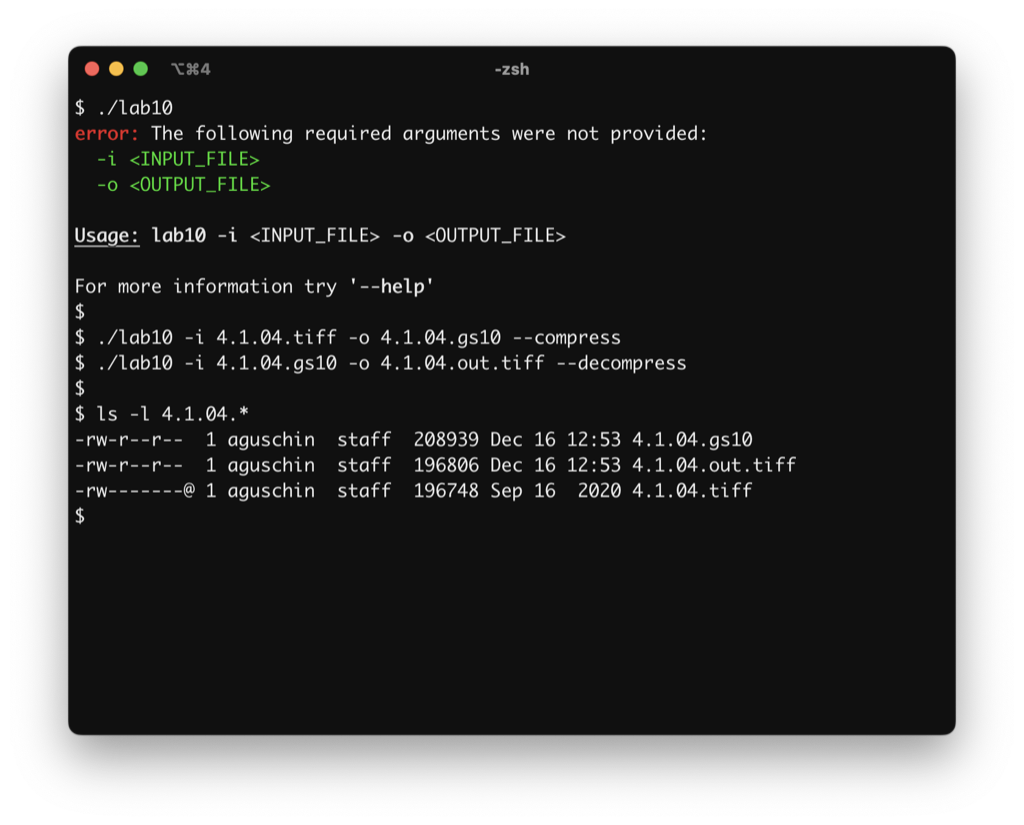
\includegraphics[width=0.9\textwidth]{test1.jpg}
  \caption{Сжатие файла 4.1.04.tiff}
  \label{fig:test_1}
\end{figure}

\begin{figure}[H]
  \centering
  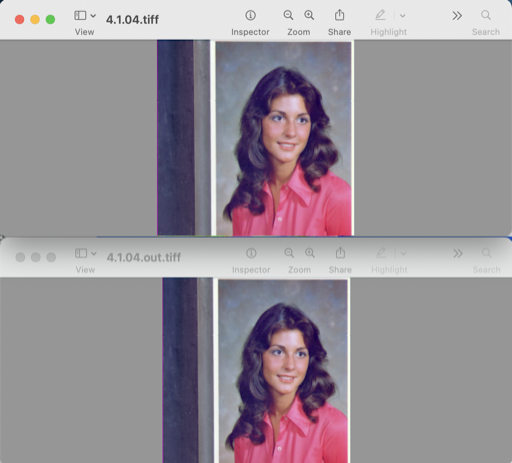
\includegraphics[width=0.9\textwidth]{test1_img.jpg}
  \caption{Сравнение разжатого изображения с 4.1.04.tiff}
  \label{fig:test_1_img}
\end{figure}


\begin{figure}[H]
  \centering
  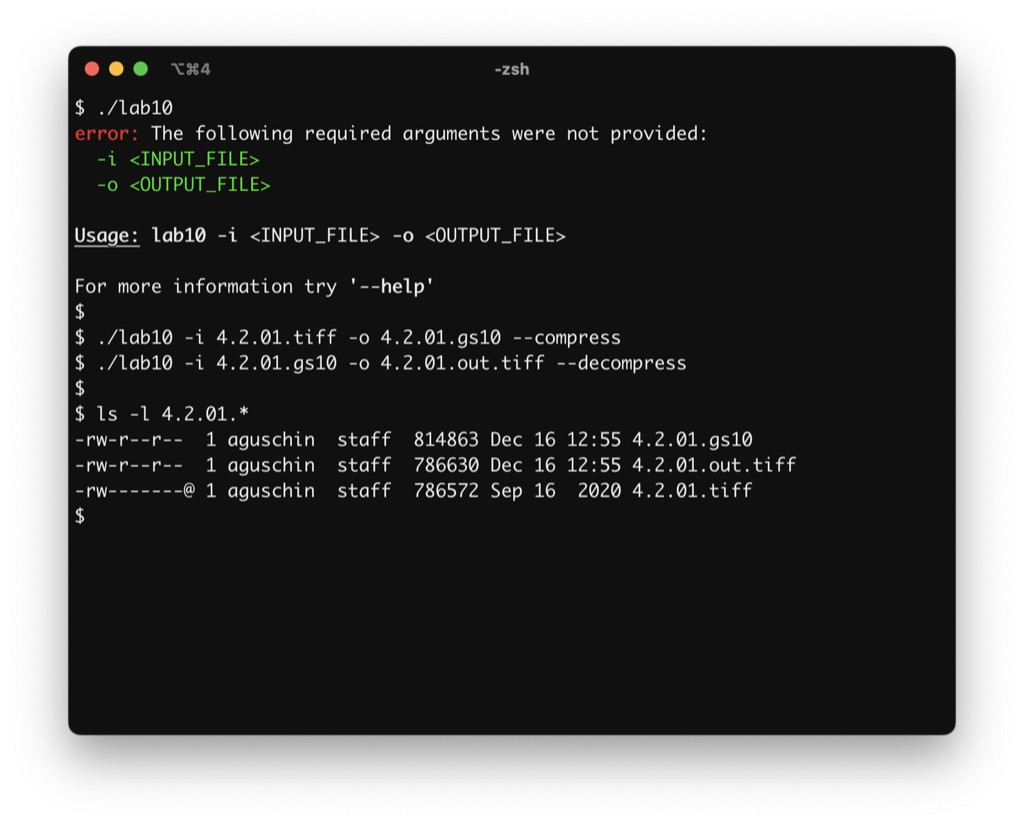
\includegraphics[width=0.9\textwidth]{test2.jpg}
  \caption{Сжатие файла 4.2.01.tiff}
  \label{fig:test_2}
\end{figure}

\begin{figure}[H]
  \centering
  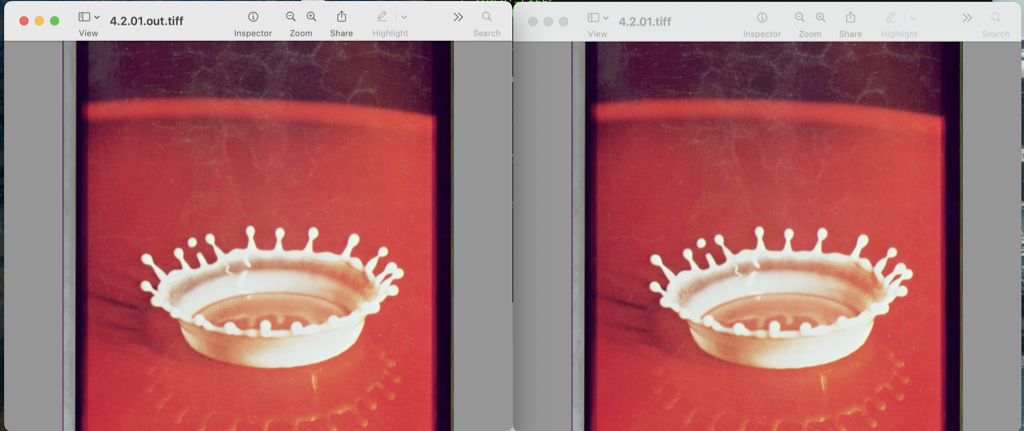
\includegraphics[width=0.9\textwidth]{test2_img.jpg}
  \caption{Сравнение разжатого изображения с 4.2.01.tiff}
  \label{fig:test_2_img}
\end{figure}


\begin{figure}[H]
  \centering
  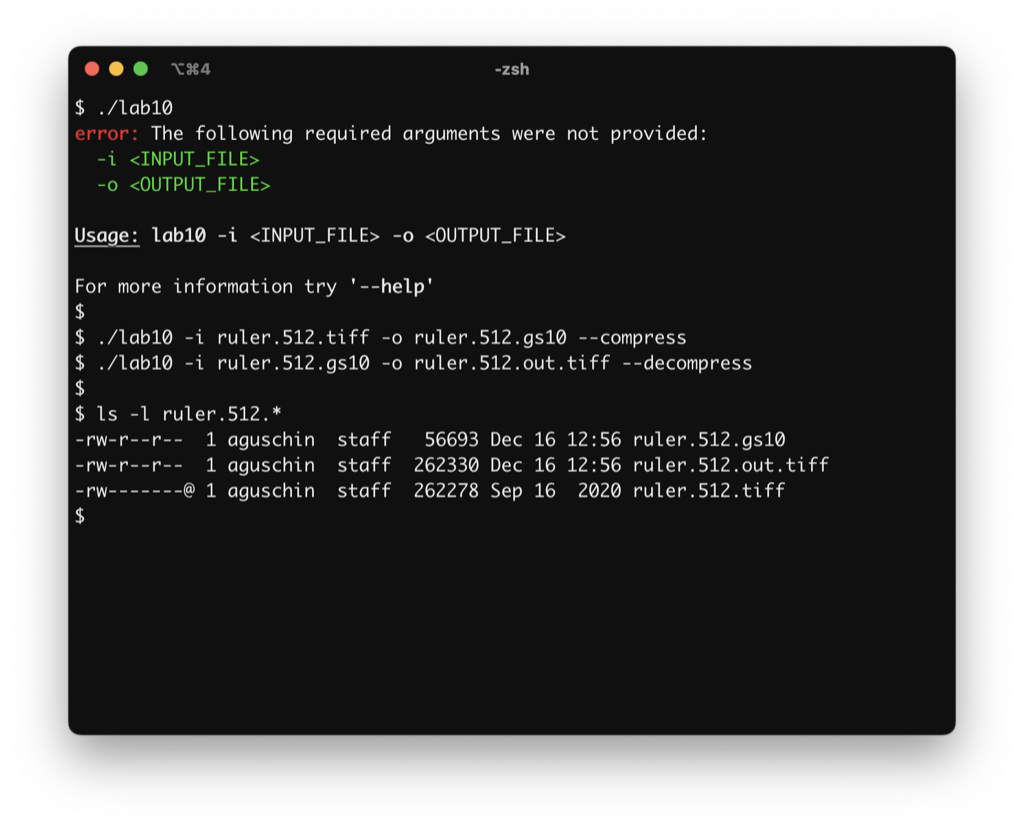
\includegraphics[width=0.9\textwidth]{test3.jpg}
  \caption{Сжатие файла ruler.512.tiff}
  \label{fig:test_3}
\end{figure}

\begin{figure}[H]
  \centering
  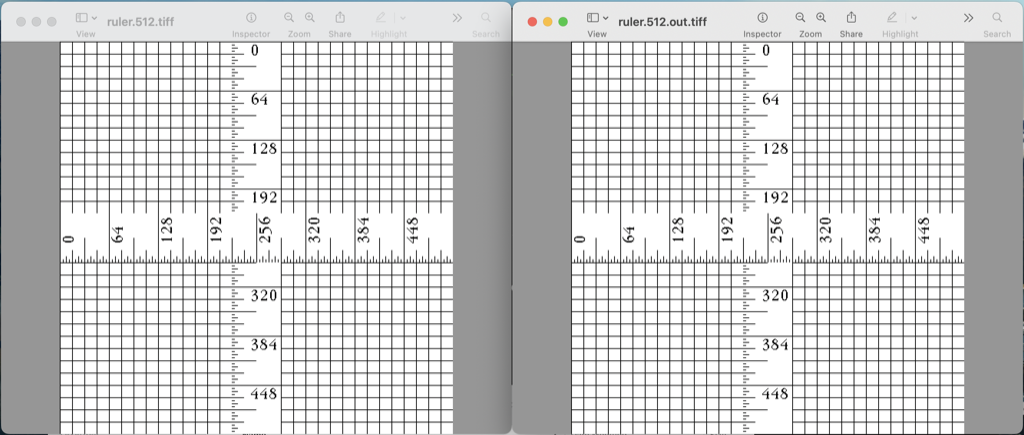
\includegraphics[width=0.9\textwidth]{test3_img.jpg}
  \caption{Сравнение разжатого изображения с ruler.512.tiff}
  \label{fig:test_3_img}
\end{figure}

\section{Вычисленные характеристики}

\subsection{Характеристика 1 (Коэффициент сжатия)}

Результаты применения программы к каждому из тестовых графических файлов занесены
в таблицу \ref{tbl:results}.

\begin{table}[H]
  \small
  \centering
  \begin{tabular}{|c|c|c|c|}
    \hline
    Название     & Исходный размер, байт & Сжатый размер, байт & Коэффициент \\ \hline \hline
    4.1.04.tiff     &  196748 &  208939 & 0.94165 \\ \hline
    4.1.05.tiff     &  196748 &  206365 & 0.9534  \\ \hline
    4.1.06.tiff     &  196748 &  202228 & 0.9729  \\ \hline
    4.1.08.tiff     &  196748 &  194291 & 1.01265 \\ \hline
    4.2.01.tiff     &  786572 &  814863 & 0.96528 \\ \hline
    4.2.03.tiff     &  786572 &  807439 & 0.97416 \\ \hline
    4.2.05.tiff     &  786572 &  831665 & 0.94578 \\ \hline
    4.2.07.tiff     &  786572 &  801443 & 0.98144 \\ \hline
    5.1.09.tiff     &   65670 &   68122 & 0.96401 \\ \hline
    5.1.11.tiff     &   65670 &   69112 & 0.9502  \\ \hline
    5.1.13.tiff     &   65670 &   13476 & 4.87311 \\ \hline
    5.1.14.tiff     &   65670 &   68240 & 0.96234 \\ \hline
    5.2.10.tiff     &  262278 &  268112 & 0.97824 \\ \hline
    5.3.01.tiff     & 1048710 & 1092262 & 0.96013 \\ \hline
    5.3.02.tiff     & 1048710 & 1087858 & 0.96401 \\ \hline
    boat.512.tiff   &  262278 &  273143 & 0.96022 \\ \hline
    gray21.512.tiff &  262278 &    6157 & 42.59834 \\ \hline
    house.tiff      &  786572 &  803252 & 0.97923 \\ \hline
    ruler.512.tiff  &  262278 &   56693 & 4.62629 \\ \hline
  \end{tabular}
  \caption{результаты тестирования}
  \label{tbl:results}
\end{table}

\subsection{Характеристика 2 (Скорость сжатия)}

Для тестирования скорости сжатия использовался произвольный графический
файл размера 4808956 байт ($\approx$4.6 мегабайта). В результате пяти
последовательных запусков, среднее время запаковки файла составило 0.05
секунды, среднее время распаковки составило 0.05 секунд.

Таким образом, средняя скорость сжатия составила 91.72356 Мбайт в секунду, а
средняя скорость разжатия составила 91.72356 Мбайт в секунду.

\subsection{Характеристика 3 (Качество сжатия)}

Качество изображения не изменилось после сжатия, так как этот алгоритм является
алгоритмом сжатия без потерь.

\section{Реализация}

Программа реализована на языке программирования Rust с использованием библиотеки
clap для чтения параметров командной строки, а также библиотеки tiff для
чтения и записи tiff файлов. Сборка производится с помощью программы cargo,
поставляющейся вместе с языком.

\subsection{Содержимое файла rle.rs}
\inputminted{rust}{../../lab10/src/rle.rs}

\subsection{Содержимое файла main.rs}
\inputminted{rust}{../../lab10/src/main.rs}

\subsection{Содержимое файла Cargo.toml}
\inputminted{toml}{../../lab10/Cargo.toml}

\end{document}
